\documentclass[10pt]{beamer}
\usepackage[utf8]{inputenc}

\usepackage{multirow,rotating}
\usepackage{color}
\usepackage{hyperref}
\usepackage{tikz-cd}
\usepackage{array}
\usepackage{siunitx}
\usepackage{amsmath, amssymb}
\usepackage{mathtools,nccmath}%
\usepackage{etoolbox, xparse} 
\usetheme{CambridgeUS}
%\usetheme{Copenhagen}



\setbeamersize{text margin left=3mm,text margin right=3mm} 

\usepackage[font=small]{caption}
\usepackage{xcolor}


\usecolortheme{dolphin}

% set colors
\definecolor{myNewColorA}{RGB}{100,149,237}
\definecolor{myNewColorB}{RGB}{100,149,237}
\definecolor{myNewColorC}{RGB}{100,149,237} % {130,138,143}
\setbeamercolor*{palette primary}{bg=myNewColorC}
\setbeamercolor*{palette secondary}{bg=myNewColorB, fg = white}
\setbeamercolor*{palette tertiary}{bg=myNewColorA, fg = white}
\setbeamercolor*{titlelike}{fg=myNewColorA}
\setbeamercolor*{title}{bg=myNewColorA, fg = white}
\setbeamercolor*{item}{fg=myNewColorA}
\setbeamercolor*{caption name}{fg=myNewColorA}
\usefonttheme{professionalfonts}
\usepackage{natbib}
\usepackage{hyperref}

\setbeamercolor{block body}{bg=structure!10}
\setbeamercolor{block title}{bg=myNewColorA}


%------------------------------------------------------------
% \titlegraphic{\includegraphics[height=0.75cm]{ua_eng_logo.png}} 





\setbeamerfont{title}{size=\large}
\setbeamerfont{subtitle}{size=\small}
\setbeamerfont{author}{size=\small}
\setbeamerfont{date}{size=\footnotesize}
\setbeamerfont{institute}{size=\footnotesize}
\title{Linear regression}%title
%\subtitle{ }%%subtitle
\author[Maria Jose Medina]{Maria Jose Medina}%%authors

\institute[USACH]{Universidad de Santiago de Chile}
\date[\textcolor{white}{September 2022}]


%------------------------------------------------------------
\AtBeginSection{
    \begin{frame}\frametitle{Table of Contents}
        \tableofcontents[currentsection]
    \end{frame}
}


\begin{document}

%The next statement creates the title page.
\frame{\titlepage}
\begin{frame}
\frametitle{Outline}
\tableofcontents
\end{frame}



\section{Multiple linear regression}
\subsection{Introduction}
\begin{frame}{Multiple regression}{Introduction}

\begin{itemize}
    \item The goal is to predict a quantitative response $Y$ on the basis of $p$ distinct predictors $x_p$. \pause

    \item It assumes that there is \textit{approximately} a relationship between $x_1, x_2, \cdots, x_p$ and $Y$ \pause
    $$ Y \approx \beta_0 + \beta_1 x_1 + \beta_2 x_3 + \cdots \beta_p x_p $$

    \item $\beta_i$ are unknown constants called \textit{model coefficients} or \textit{parameters}. \pause

    \item Let $\hat{y_i} = \hat{\beta}_0 + \hat{\beta}_1 x_1 + \cdots + \hat{\beta}_p x_p $ be the prediction for $Y$ based on the predictors of $x_p$. \pause \\ Then 
    $$e_i = y_i - \hat{y}_i$$ \pause 
    represents the $i$th \textbf{residual}.
      
\end{itemize}
\end{frame}


\subsection{Estimating the model coefficients}
\begin{frame}{Multiple regression}{Estimating the model coefficients}


\begin{itemize}
    \item Using \textit{residuals}, we define the \textbf{residual sum of squares}(RSS) as \pause

    \begin{align*}
      RSS &=  e_1^2 + e_2^2 + \cdots e_n^2   \\
          &= \sum_{i=1}^n (y_i - \hat{\beta}_0 - \hat{\beta}_1 x_{i1} -  \hat{\beta}_2 x_{i2} - \hat{\beta}_p x_{ip} )^2
    \end{align*}  \pause

    \item To estimate the coefficients we use the \textbf{least squares approach}, in which we seek to minimize RSS.  \pause

    \begin{columns}
         \column{0.50\linewidth}
         \hspace{0.5cm} $$ \hat{\beta} = (X'X)^{-1} X'y  $$  
           \column{0.50\linewidth}
            \centering
        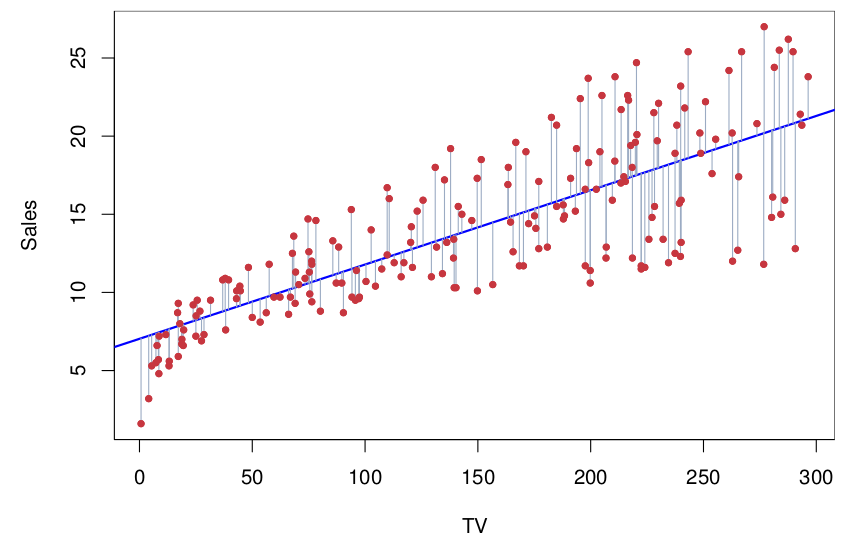
\includegraphics[height=4cm, width=4cm]{multiple-lr/ols.png}
    \end{columns} 

\end{itemize}

\end{frame}



\subsection{Some important questions}
\begin{frame}{Multiple regression}{Some important questions}
Now we have to evaluate the model:
\begin{enumerate}
    \item <1-> Is at least one of the predictors $x_1, x_2, \cdots x_n$ useful in predicting the response? \pause    
    \item <2-4> Do all the predictors help to explain $Y$, or is only a subset of the predictors useful? \pause
    \item <3-4> How well does the model fit the data? \pause
    \item <4>Given a set of predictor values, what response value should we predict, and how accurate is our prediction? \pause 
\end{enumerate}
\end{frame}


%%%%%%%%%%%%%%%%%% QUESTION 1 %%%%%%%%%%%%%%%%%5
\begin{frame}{Important questions}{One: Is There a Relationship Between the Response and Predictors?}

\begin{itemize}
    \item In simple linear regression ($y = \beta_0 + \beta_1 x$), we simply check whether $\beta_1 = 0$ through hypothesis testing. \pause
    \item Here, we extend that idea with $p$ predictors. \pause
    \item We need to ask:
    \begin{enumerate}
        \item Are all regression coefficients zero? \pause
        \item Are only a particular subset of regression coefficients zero?
    \end{enumerate}

    \end{itemize}

\end{frame}

\begin{frame}{Important questions}{One: Is There a Relationship Between the Response and Predictors? \\ - Are all regression coefficients zero? }

To know whether all of the regression coefficients are zero, i.e. $\beta_1 = \beta_2 = \cdots = \beta_p = 0.$, we test the null hypothesis, 

$$H_0: \beta_1 = \beta_2 = \cdots = \beta_p = 0 $$ 

versus the alternative \pause

$$H_a: \text{ at least one } \beta_j \text{ is non-zero}.$$

This hypothesis test is performed by computing the \textbf{F-statistic}.
    
\end{frame}


\begin{frame}{Important questions}{One: Is There a Relationship Between the Response and Predictors? \\ - Are all regression coefficients zero? }

Assuming homoscedasticity, the F-statistic is given by, 

$$F = \frac{ (TSS - RSS)/p   }{RSS/(n-p-1)},$$

where \pause

\begin{itemize}
    \item $TSS = \sum(y_i - \bar{y})^2$ is the \textbf{total sum of squares}. Measures the total variance in the response $Y$ , and can be thought of as the amount of variability inherent in the response before the regression is performed. \pause
    \item $RSS = \sum(y_i - \hat{y}_i)^2$ is the \textbf{residual sum of squares}. Measures the amount of variability that is left unexplained after performing the regression. \pause
    \item $TSS - RSS \rightarrow$ is the amount of variability in the response that is explained (or removed) by performing the regression. \pause

\end{itemize}

\end{frame}

\begin{frame}{Important questions}{One: Is There a Relationship Between the Response and Predictors? \\ - Are all regression coefficients zero? }

\begin{itemize}
    \item If we assume homoscedasticity then, \\ $\mathbb{E} \{  RSS / (n-p-1)  \} = \sigma^2$  \pause 
    \item Assuming that $H_0$ is true, then \\ $\mathbb{E} \{  (TSS - RSS) / p  \} = \sigma^2$.  \pause 

    \item Therefore, \textcolor{blue}{if $H_0$ is true} (i.e. there is no relationship between $x_1, \cdots x_p$ and $Y$), \textcolor{blue}{F-statistic is closer to $1$.} \pause

    \item On other hand, if $H_0$ is not true, \\
    $\mathbb{E} \{  (TSS - RSS) / p  \} > \sigma^2 \Rightarrow F > 1$ \pause

    \item How large does the F-statistic need to be before we can reject $H_0$ and conclude that there is a relationship? \pause \\ 
    $\rightarrow$ It depends on the values of $n$ and $p$. 
 
\end{itemize}
    
\end{frame}


\begin{frame}{Important questions}{One: Is There a Relationship Between the Response and Predictors? \\ - Are all regression coefficients zero? }

When $n$ is large, \pause

\begin{itemize}
    \item F-statistic approximately follows
an F-distribution, even if the errors are not normally distributed. \pause

    \item a F-statistic that is just a little larger than $1$ might still provide evidence against $H_0$.
\end{itemize} \pause

When $n$ is small, \pause

\begin{itemize}
    \item A larger F-statistic is is needed to reject $H_0$. \pause
\end{itemize}

For any value $n$ and $p$, \pause
\begin{itemize}

    \item Compute the $p-value$: The p-value indicates how likely it is to observe the results due to chance, assuming $H_0$. \pause
        \begin{itemize}
            \item Small p-value: very unlikely that $H_0$ is true $\rightarrow$ \textcolor{blue}{Reject $H_0$}. \pause
            \item Large p-value: very likely that $H_0$ is true $\rightarrow$ \textcolor{blue}{Fail to reject $H_0$.} \pause 
        \end{itemize}
    
\end{itemize}

Typical p-value cutoffs for rejecting the null hypothesis are $5\%$ or $1\%$.
    
\end{frame}


\begin{frame}{Important questions}{One: Is There a Relationship Between the Response and Predictors? \\ - Are only a particular subset of regression coefficients zero?}

Sometimes we want to test the hypothesis if a particular subset $q$ of the coefficients are zero, \pause
$$H_0: \beta_{p-q+1} = \beta_{p-q+2} = \cdots = \beta_p = 0$$ \pause
versus the alternative, \pause
$$H_a: \text{ One or more than } q \text{ restrictions assuming } H_0 \text{ does not stand}. $$  \pause

To test the hypothesis: \pause
\begin{itemize}
    \item Fit a regression model $y_0$ that uses all variables except $q$. \pause
    \item Calculate the residual sum of squares for that model, $RSS_0$. \pause
    \item Compute the appropiate F-statistic
    $$F = \frac{(RSS_0 - RSS)/q}{RSS/(n-p-1)}.$$ \pause
    \item Compute p-values.
    
\end{itemize}



\end{frame}

\begin{frame}{Important questions}{One: Is There a Relationship Between the Response and Predictors? \\ - Are only a particular subset of regression coefficients zero?}

    \begin{itemize}
        \item The approach of using an F -statistic to test for any association between the predictors and the response works when $p$ is relatively small compared to $n$. \pause
        \item If $p > n$ then there are more coefficients $\beta_j$ to estimate than observations from which to estimate them. \pause
        \item We cannot even fit the multiple linear regression model using least squares, so the \textbf{F-statistic cannot be used}. 
    \end{itemize}

    
\end{frame}


%%%%%%%%%%%%%%%%%%%%% OUTLINE %%%%%%%%%%%%%%%%%%%
\begin{frame}[noframenumbering]{Multiple regression}{Some important questions}

\begin{enumerate}
    \item<1> Is at least one of the predictors $x_1, x_2, \cdots x_n$ useful in predicting the response?  
    \item<1-2> Do all the predictors help to explain $Y$, or is only a subset of the predictors useful? 
    \item<1> How well does the model fit the data? 
    \item<1> Given a set of predictor values, what response value should we predict, and how accurate is our prediction?
    
\end{enumerate}
\end{frame}

%%%%%%%%%%%%%%%%%% QUESTION 2 %%%%%%%%%%%%%%%%%5
\begin{frame}{Important questions}{Two: Deciding on Important Variables}

Ideally, we would like to perform \textbf{variable selection} by trying out a lot of different models, each containing a different subset of the predictors. \pause For example, if $p=2$, then we can consider, \pause

\begin{enumerate}
    \item A model containing no variables, \pause
    \item A model containing $x_1$ only, \pause
    \item A model containing $x_2$ only, and \pause
    \item A model containing both $x_1$ and $x_2$. \pause   
\end{enumerate}

Then we can use Akaike information criterion (AIC), Bayesian information criterion (BIC), and adjusted $R^2$ to select the best model. \pause \\

Unfortunately, there are a \textcolor{blue}{total of $2^p$ models} that contain subsets of $p$ variables. \pause  \\

\begin{itemize}
    \item If if $p = 2$, then there are $2^2 = 4$ models to consider. \pause
    \item if $p = 30$, then we must consider $2^{30} = 1.073.741.824$ models! \\ \pause $\rightarrow$ \textbf{This is not practical!}
\end{itemize}


\end{frame}


\begin{frame}{Two: Deciding on Important Variables}

So when $p$ is not small, we can consider these automated approaches: \pause

\begin{itemize}
    \item \textbf{Forward selection} \pause
     \begin{enumerate}
            \item We begin with by fitting the \textit{null model} $y_0$. \pause
            \item Fit $p$ simple linear regressions and compute its RSS. \pause
            \item Add to the null model the variable that results in the lowest RSS, this create a new model $y_1$. \pause
            \item Repeat the step $2$ and $3$ but now with $p-1$ regressors. \pause
            \item Continue until some stopping rule is satisfied. \pause
        \end{enumerate}

    \item \textbf{Backward selection} \pause
     \begin{enumerate}
            \item We start with all the variables in the model $y_p$. \pause
            \item Remove the variable with the largest p-value. \pause
            \item The new $(p - 1)$-variable model is fit, and the variable with the largest p-value is removed. \pause
            \item Continue until some stopping rule is satisfied. 
        \end{enumerate}
        
\end{itemize}
    
\end{frame}


\begin{frame}{Two: Deciding on Important Variables}

\begin{itemize}
    \item \textbf{Mixed selection}: a combination of forward and backward selection. \pause
    \begin{enumerate}
        \item We start with the null model and then we successively add the variables that provides the best fit (lowest RSS). \pause
        \item If at any point the p-value for one of the variables in the model rises above a certain threshold, remove that variable. \pause
        \item We continue to perform these forward and backward steps until all variables in the model have a sufficiently low p-value, and all variables outside the model would have a large p-value if added to the model. \pause
    \end{enumerate}
\end{itemize}

Important notes: \pause
\begin{itemize}
    \item Backward selection cannot be used if $p > n$. \pause
    \item Forward selection can always be used but might include variables early that later become redundant. \pause
    \item Mixed selection can remedy redundant variables.
\end{itemize}

        
\end{frame}


%%%%%%%%%%%%%%%%%%%%% OUTLINE %%%%%%%%%%%%%%%%%%%
\begin{frame}[noframenumbering]{Multiple regression}{Some important questions}

\begin{enumerate}
    \item<1> Is at least one of the predictors $x_1, x_2, \cdots x_n$ useful in predicting the response?  
    \item<1> Do all the predictors help to explain $Y$, or is only a subset of the predictors useful? 
    \item<1-2> How well does the model fit the data? 
    \item<1> Given a set of predictor values, what response value should we predict, and how accurate is our prediction?
    
\end{enumerate}
\end{frame}

%%%%%%%%%%%%%%%%%%%%%% QUESTION 3 %%%%%%%%%%%%%%%%%
\begin{frame}{Important questions}{Three: Model fit}

The quality of a linear regression fit is typically assessed using two related quantities: \pause

\begin{enumerate}
    \item Residual standard error (RSE) \pause
    \item $R^2$ statistic.
 
\end{enumerate}
\end{frame}


\begin{frame}{Important questions}{Three: Model fit - Residual standard error (RSE)}

\begin{itemize}
    \item Recall that from every model, there is some error term $\epsilon$ associated with each observation. \pause

    \item The RSE is an estimate of the standard
deviation of $\epsilon$. \pause

    \item Roughly speaking, it is the average amount that the response will deviate from the true regression line. \pause
  
\end{itemize}

\begin{align*}
    RSE &= \sqrt{\frac{1}{n-2} RSS} = \sqrt{\frac{1}{n-2} \sum_{i=1}^n (y_i - \hat{y}_i)^2}
\end{align*} \pause

\begin{itemize}
    \item If $\hat{y}_i \approx y_i \, \forall i \in n$, then RSE is small. $\rightarrow$ \textcolor{blue}{The model fits the data well.} \pause

    \item If $\hat{y}_i$ is very far from $y_i$ for one or more observations, then RSE may be quite large. $\rightarrow$ \textcolor{blue}{The model doesn’t fit the data well.}
\end{itemize}


\end{frame}


\begin{frame}{Important questions}{Three: Model fit - $R^2$ statistic}


\begin{itemize}
    \item The $R^2$ it's the proportion of variance explained. \pause
    \item It always takes on a value between 0 and 1, and is independent of the scale of $Y$. \pause
\end{itemize}

$$R^2 = \frac{TSS - RSS}{TSS} = 1 - \frac{RSS}{TSS}$$

\begin{itemize}
    \item \textcolor{blue}{TSS} measures the \textcolor{blue}{total variance in $Y$} \pause % and can be thought of as the amount of variability inherent in the response before the regression is performed.
    \item \textcolor{blue}{RSS} measures the \textcolor{blue}{variability that is left unexplained} after performing the regression. \pause
    \item \textcolor{blue}{TSS - RSS} is the amount of \textcolor{blue}{variability in $Y$ that is explained} (or removed) by performing the regression. \pause
    \item $R^2$ measures the proportion of variability in $Y$ that can be explained using $X$. \pause
\end{itemize}

\end{frame}


%%%%%%%%%%%%%%%%%%%%% OUTLINE %%%%%%%%%%%%%%%%%%%
\begin{frame}[noframenumbering]{Multiple regression}{Some important questions}

\begin{enumerate}
    \item<1> Is at least one of the predictors $x_1, x_2, \cdots x_n$ useful in predicting the response?  
    \item<1> Do all the predictors help to explain $Y$, or is only a subset of the predictors useful? 
    \item<1> How well does the model fit the data? 
    \item<1-2> Given a set of predictor values, what response value should we predict, and how accurate is our prediction?
    
\end{enumerate}
\end{frame}


\begin{frame}{Important questions}{Four: Predictions}

The accuracy of our predictions depends on three sorts of uncertainty: \pause

\begin{enumerate}
    \item \textbf{The reducible error} 
    \\ $\rightarrow$ Related to the inaccuracy in the coefficient estimates.  \pause 
    \\ $\rightarrow$ We compute a confidence interval in order to determine how close $\hat{Y}$ will be to $f(X)$. \pause

    \item \textbf{Model bias} \pause 
    \\ $\rightarrow$ Assuming a linear model for $f(X)$ is an approximation of reality. \pause

    \item \textbf{The irreducible error.} \pause \\
    $\rightarrow$ We use \textcolor{blue}{prediction intervals} to answer how much will $\hat{Y}$ vary from $Y$. \pause \\
    $\rightarrow$  Prediction intervals are always wider than confidence intervals.
    
\end{enumerate}
    
\end{frame}



\section{Other considerations in the Regression model}
\subsection{Qualitative predictors}
\begin{frame}{Other considerations in the Regression model}{Qualitative predictors: Predictors with only two levels}

\begin{itemize}
    \item Suppose that we wish to investigate differences in credit card balance between people who own a house vs those who don't. \pause
    \item We can adding the qualitative predictor to the regression as a \textcolor{blue}{dummy variable}. \pause 
        \begin{equation*}
        x_i = 
        \begin{cases} 
            1 & \text{ if $i$th person owns a house,}\\
            0 & \text{ if $i$th person does not own a house,}
        \end{cases}
    \end{equation*}

    \item This results in the model,
    \begin{equation*}
        y_i = \beta_0 + \beta_1 x_i + \epsilon_i = 
        \begin{cases}
              \beta_0 + \beta_1 + \epsilon_i & \text{if $i$th person owns a house,} \\
                 \beta_0 + \epsilon_i & \text{if $i$th person does not.}
        \end{cases}
    \end{equation*}
\end{itemize}

\end{frame}

\begin{frame}{Other considerations in the Regression model}{Qualitative predictors}
    
    \begin{equation*}
        y_i = \beta_0 + \beta_1 x_i + \epsilon_i = 
        \begin{cases}
              \beta_0 + \beta_1 + \epsilon_i & \text{if $i$th person owns a house,} \\
                 \beta_0 + \epsilon_i & \text{if $i$th person does not.}
        \end{cases}
    \end{equation*}

\begin{itemize}
    \item $\beta_0$ is the average credit card balance among those who do not own a house. \pause
    \item $\beta_0 + \beta_1$ is the average credit card balance among those who do own their house. \pause
    \item $\beta_1$ is the average difference in credit card balance between owners and non-owners. \pause
    \item To test significance, we test $H_0: \beta_1 = 0$ \pause
\end{itemize}

\begin{block}{Note}
    $\rightarrow$ The decision to code owners as 1 and non-owners as 0 is arbitrary, and has no effect on the regression fit. \pause \\
    $\rightarrow$ That decision only alter the interpretation of the coefficients.
\end{block}


\end{frame}


\begin{frame}{Other considerations in the Regression model}{Qualitative predictors: Predictors with More that Two Levels}

\begin{itemize}
    \item Suppose now that we want to investigate differences in credit card balance between people who lives in one of these \textbf{regions}: South, West, East. \pause
    \item Single dummy variable cannot represent all possible values, so we create additional ones. \pause

\begin{equation*}
        x_{i1} = 
        \begin{cases} 
            1 & \text{ if $i$th person is from the South,}\\
            0 & \text{ if $i$th person is not from the South,}
        \end{cases}
    \end{equation*}

\begin{equation*}
        x_{i2} = 
        \begin{cases} 
            1 & \text{ if $i$th person is from the West,}\\
            0 & \text{ if $i$th person is not from the West,}
        \end{cases}
    \end{equation*}
    \item This results in the model, \pause

\begin{equation*}
        y_i = \beta_0 + \beta_1 x_{i1} + \beta_{i2} + \epsilon_i = 
        \begin{cases}
        \beta_0 + \beta_1 + \epsilon_i & \text{if $i$th person is from the South,} \\
        \beta_0 + \beta_2 + \epsilon_i & \text{if $i$th person is from the West,} \\
        \beta_0 + \epsilon_i & \text{if $i$th is from the East.}
        \end{cases}
\end{equation*}
    
\end{itemize}

\end{frame}


\begin{frame}{Other considerations in the Regression model}{Qualitative predictors: Predictors with More that Two Levels}

\begin{equation*}
        y_i = \beta_0 + \beta_1 x_{i1} + \beta_{i2} + \epsilon_i = 
        \begin{cases}
        \beta_0 + \beta_1 + \epsilon_i & \text{if $i$th person is from the South,} \\
        \beta_0 + \beta_2 + \epsilon_i & \text{if $i$th person is from the West,} \\
        \beta_0 + \epsilon_i & \text{if $i$th is from the East.}
        \end{cases}
\end{equation*}

\begin{itemize}
    \item $\beta_0$ is the average credit card balance for individuals from the East. \pause
    \item $\beta_1$ is the difference in the average balance between people from the South versus the East. \pause
    \item $\beta_2$ is the difference in the average balance between those from the West versus the East.
\end{itemize}

\begin{block}{Notes}
    $\rightarrow$ The level selected as the baseline category is arbitrary, and the final predictions for each group will be the same regardless of this choice. \\ \pause
    $\rightarrow$ The coefficients and their p-values \textbf{do depend} on the choice of dummy variable coding. \\ \pause
    $\rightarrow$ To test significance, we can use F-test on $H_0: \beta_1 = \beta_0 = 0$. \textbf{This does not depend on the coding}. 
\end{block}

\end{frame}

\subsection{Removing additive assumption}
\begin{frame}{Other considerations in the Regression model}{Removing the Additive Assumption}

Consider the standard linear regression model with two variables, 
        $$Y = \beta_0 + \beta_1 X_1 + \beta_2 + \epsilon$$
According to this, \pause
\begin{itemize}
    \item A one-unit increase in $X_1$ is associated with an average increase in $Y$ of $\beta_1$ units. \pause
    \item Notice that the presence of $X_2$ does not alter this statement. \pause
    \item We can extend this model to include an \textbf{interaction term} with $X_1$ and $X_2$. \pause 
    \begin{equation*}
        Y = \beta_0 + \beta_1 X_1 + \beta_2 X_2 + \beta_3 X_1 X_2 + \epsilon.
    \end{equation*}
    \item \pause Now $Y$ can be rewritten as, 
    \begin{align*}
        Y &=   \beta_0 + (\beta_1 X_1 + \beta_3 X_2)X_1 + \beta_2 X_2 + \epsilon \\
        Y &=   \beta_0 + \Tilde{\beta_1}X_1 + \beta_2 X_2 + \epsilon \\
        & \text{with } \Tilde{\beta_1} = \beta_1 + \beta_3 X_2. 
    \end{align*} 
\end{itemize}
    
\end{frame}

\begin{frame}{Other considerations in the Regression model}{Removing the Additive Assumption}

    \begin{align*}
        Y &=   \beta_0 + (\beta_1 X_1 + \beta_3 X_2)X_1 + \beta_2 X_2 + \epsilon \\
        Y &=   \beta_0 + \Tilde{\beta_1}X_1 + \beta_2 X_2 + \epsilon \\
         & \text{with } \Tilde{\beta_1} = \beta_1 + \beta_3 X_2.
    \end{align*}

\begin{itemize}
    \item Since $\Tilde{\beta_1}$ is now a function of $X_1$, the association between $X_1$ and $Y$ is no longer constant. \pause
    \item A change in the value of $X_2$ will change the association between $X_1$ and $Y$. \pause
    \item Similarly, a change in the value of $X_1$ changes the association between $X_2$ and $Y$.\pause
\end{itemize}
\end{frame}

\begin{frame}{Other considerations in the Regression model}{Removing the Additive Assumption}

    \begin{align*}
        Y &=   \beta_0 + (\beta_1 X_1 + \beta_3 X_2)X_1 + \beta_2 X_2 + \epsilon \\
        Y &=   \beta_0 + \Tilde{\beta_1}X_1 + \beta_2 X_2 + \epsilon \\
        & \text{with } \Tilde{\beta_1} = \beta_1 + \beta_3 X_2.
    \end{align*}
    

\begin{block}{The hierarchical principle}
        If we include an \textbf{interaction} in a model, we should also include the \textbf{main effects}, even if the p-values associated with principle their coefficients are not significant.
\end{block} \pause
Why? \pause
\begin{itemize}
    \item If $X_1 \times X_2$ is related to the response, then whether or not the coefficients of $X_1$ or $X_2$ are exactly zero is of little interest. \pause
    \item $X_1 \times X_2$ is typically correlated with $X_1$ and $X_2$, and so leaving them out tends to alter the meaning of the interaction. \pause
\end{itemize}
    
\end{frame}


    



\subsection{Potential problems}
\begin{frame}{Potential Problems}

When we fit a linear regression model to a particular data set, many problems may occur. Most common among these are the following:

%%%%%%%%%%%%%%%%%%%%%%%% OUTLINE %%%%%%%%%%%%%%%%%%%%%%%%%%%%%%

\begin{enumerate}
    \item<1-2> Non-linearity of the response-predictor relationships.
    \item<1> Correlation of error terms.
    \item<1> Non-constant variance of error terms.
    \item<1> Outliers.
    \item<1> High-leverage points.
    \item<1> Collinearity.
\end{enumerate}
    
\end{frame}

\begin{frame}{Potential Problems}{Non-linearity of the Data}

    
\begin{itemize}
    \item The linear regression model assumes that there is a straight-line relationship between the predictors and the response. \pause
    
    \item If the true relationship is far from linear, then virtually all of the conclusions that we draw from the fit are suspect. \pause

    \item \textit{Residual plots} are a useful graphical tool for identifying non-linearity. 

    \item In the case of a multiple regression model, we plot the residuals versus the predicted (or fitted) values $\hat{y}_i$. 


    \end{itemize}

\end{frame}

\begin{frame}{Potential Problems}{Non-linearity of the Data}

\begin{itemize}
    \item Ideally, the residual plot will show no fitted discernible pattern. \pause

    \item The presence of a pattern may indicate a problem with some aspect of the linear model. \pause
\end{itemize}

\begin{columns}

    \column{0.4\linewidth}    
    \begin{figure}[!h]
        \centering
        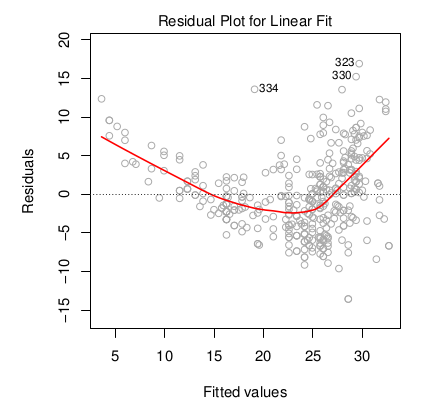
\includegraphics[height=4cm, width=4cm]{other-lr/residual_fit.png}
    \end{figure} \pause

    \column{0.4\linewidth}    

    \begin{block}{Note}
    If the residual plot indicates that there are non-linear associations in the data, then a simple approach is to use \textbf{non-linear transformations} of the predictors, such as log$X$ and $\sqrt{X}$, in the regression model. 
    \end{block}
    
    
\end{columns}
    
\end{frame}    

%%%%%%%%%%%%%%%%%%%%%%%% OUTLINE %%%%%%%%%%%%%%%%%%%%%%%%%%%%%%

\begin{frame}[noframenumbering]{Potential Problems}


\begin{enumerate}
    \item<1> Non-linearity of the response-predictor relationships.
    \item<1-2> Correlation of error terms.
    \item<1> Non-constant variance of error terms.
    \item<1> Outliers.
    \item<1> High-leverage points.
    \item<1> Collinearity.
\end{enumerate}
    
\end{frame}

\begin{frame}{Potential Problems}{Correlation of Error Terms}

\begin{itemize}
    \item An important assumption of the linear regression model is that the error terms, $\epsilon_1, \epsilon_2, \cdots, \epsilon_n$, are uncorrelated. \pause \\
    $\rightarrow$ i.e. the fact that $\epsilon_i$ is positive provides little or no information about the sign of $\epsilon_{i+1}$. \pause

    \item Is there is correlation among the error terms, then the estimated standard errors will tend to underestimate the true standard errors. \pause
    
    \item As a result, confidence and prediction intervals will be narrower than they should be. \pause

    \item In addition, p-values associated with the model will be lower than they should be; this could cause us to erroneously conclude that a parameter is statistically significant. \pause

    \item Why might correlations among the error terms occur? \pause \\ $\rightarrow$ Such correlations frequently occur in the context of \textbf{time series data}.
    
\end{itemize}


\end{frame}

\begin{frame}{Potential Problems}{Correlation of Error Terms}

\begin{itemize}
    \item In order to determine if this is the case for a given data set, we can plot the residuals from our model as a function of time. \pause

    \item If the errors are \textcolor{blue}{uncorrelated}, then there should be \textcolor{blue}{no discernible pattern}. \pause

    \item If the error terms are \textcolor{blue}{positively correlated}, then we may see \textcolor{blue}{tracking} in the residuals. \pause $\rightarrow$ adjacent residuals may have similar values. \pause

    
    \begin{figure}[!h]
    \centering
    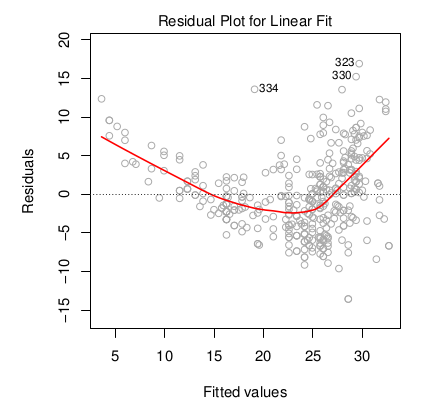
\includegraphics[height=4cm, width=7.5cm]{other-lr/residual_fit.png}
    \end{figure} \pause
    \item Good experimental design is crucial in order to mitigate the risk of such correlations.
    
\end{itemize}

    
\end{frame}


\begin{frame}[noframenumbering]{Potential Problems}


\begin{enumerate}
    \item<1> Non-linearity of the response-predictor relationships.
    \item<1> Correlation of error terms.
    \item<1-2> Non-constant variance of error terms.
    \item<1> Outliers.
    \item<1> High-leverage points.
    \item<1> Collinearity.
\end{enumerate}
    
\end{frame}

\begin{frame}{Potential Problems}{Non-constant Variance of Error Terms}

\begin{itemize}
    \item Another important assumption of the linear regression model is that the error terms have a constant variance, $Var(\epsilon_i ) = \sigma^2$ \pause

    \item One can identify non-constant variances in the errors, or \textcolor{blue}{heteroscedasticity}, from the presence of a funnel shape in the residual plot. \pause

    \item When faced with this problem, one possible solution is to transform the response $Y$ using a \textbf{concave} function  such as $log(Y)$ or $\sqrt{Y}$. \pause

    \item Such a transformation results in a greater amount of shrinkage of the larger responses, leading to a reduction in heteroscedasticity. \pause

\end{itemize}
    
\end{frame}

\begin{frame}{Potential Problems}{Non-constant Variance of Error Terms}

    \begin{figure}[!h]
    \centering
    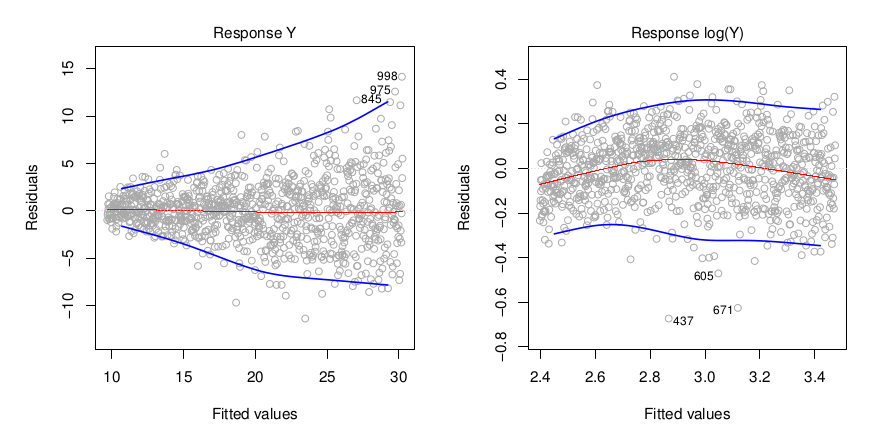
\includegraphics[height=6cm, width=9.5cm]{other-lr/heteroscedasticity.png}
    \end{figure} 
    
\end{frame}


\begin{frame}[noframenumbering]{Potential Problems}


\begin{enumerate}
    \item<1> Non-linearity of the response-predictor relationships.
    \item<1> Correlation of error terms.
    \item<1> Non-constant variance of error terms.
    \item<1-2> Outliers.
    \item<1> High-leverage points.
    \item<1> Collinearity.
\end{enumerate}
    
\end{frame}

\begin{frame}{Potential Problems}{Outliers}

    \begin{itemize}
        \item An outlier is a point for which $yi$ is far from the value predicted by the outlier model. \pause

        \item Include outliers in the regression fit can cause alterations on the RSE values, which are further used to compute confidence intervals and p-values. \pause

        \item A single data point can have implications for the interpretation of the fit. \pause

        \item To identify outliers, we can compute the \textbf{studentized residuals} by dividing each residual $e_i$ by its estimated standard error. \pause

        \item Observations whose studentized residuals are greater than 3 in absolute value are possible outliers. \pause
        
    \end{itemize}

\end{frame}

\begin{frame}{Potential Problems}{Outliers}
    \begin{figure}
        \centering
        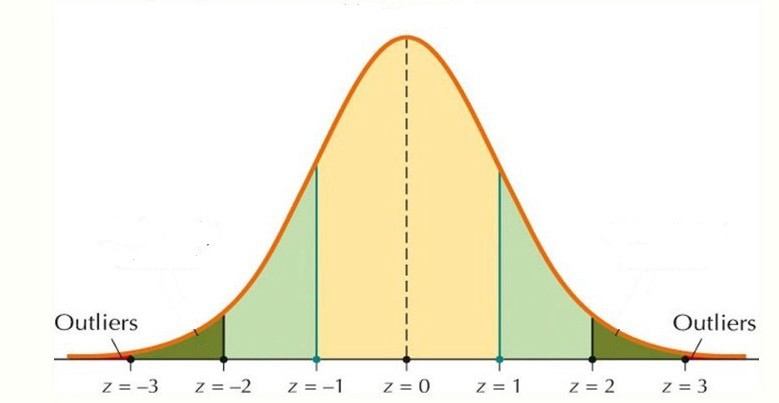
\includegraphics[height=5cm, width=8.5cm]{other-lr/outlier.jpeg}
    \end{figure}

    \begin{block}{Notes}
        \begin{itemize}
            \item If we believe that an outlier has occurred due to an error in data collection or recording, then one solution is to simply remove the observation. \pause
            \item However, care should be taken, since an outlier may instead indicate a deficiency with the model, such as a missing predictor.
    \end{itemize}            
    \end{block}
\end{frame}


%%%%%%%%%%%%%%%%%%%% OUTLINE %%%%%%%%%%%%%%%%%%%%%%%%
\begin{frame}[noframenumbering]{Potential Problems}


\begin{enumerate}
    \item<1> Non-linearity of the response-predictor relationships.
    \item<1> Correlation of error terms.
    \item<1> Non-constant variance of error terms.
    \item<1> Outliers.
    \item<1-2> High-leverage points.
    \item<1> Collinearity.
\end{enumerate}
    
\end{frame}

\begin{frame}{Potential Problems}{Outliers}

\begin{itemize}
    \item We just saw that outliers are observations for which the response $y_i$ is unusual given the predictor $x_i$. \pause 
    
    \item In contrast, observations with \textbf{high leverage} have an \textbf{unusual value for $x_i$}. \pause
    
    \item High leverage observations tend to have a sizable impact on the estimated regression line. \pause
    
    \item In order to quantify an observation’s leverage, we compute the \textcolor{blue}{leverage statistic}: \pause

    $$h_i = \frac{1}{n} + \frac{(x_i - \Bar{x})^2}{\sum_{i'=1}^n (x_i' - \Bar{x})^2 }$$ \pause

    \end{itemize}
    \end{frame}

\begin{frame}{Potential Problems}{Outliers}

$$h_i = \frac{1}{n} + \frac{(x_i - \Bar{x})^2}{\sum_{i'=1}^n (x_i' - \Bar{x})^2 }$$ \pause

\begin{itemize}

    \item A large value of this statistic indicates an observation with high leverage.
    
\end{itemize}

\begin{block}{Notes}
    $\rightarrow$ $h_i$ increases with the distance of $x_i$ from $\Bar{x}$. \pause  \\

    $\rightarrow$ The average leverage for all the observations is always equal to $(p + 1)/n$. \pause \\
    
    $\rightarrow$ If a given observation has a leverage statistic that greatly exceeds $(p+1)/n$, then we may suspect that the corresponding point has high leverage.   
\end{block}
    
    
\end{frame}


\begin{frame}[noframenumbering]{Potential Problems}


\begin{enumerate}
    \item<1> Non-linearity of the response-predictor relationships.
    \item<1> Correlation of error terms.
    \item<1> Non-constant variance of error terms.
    \item<1> Outliers.
    \item<1> High-leverage points.
    \item<1-2> Collinearity.
\end{enumerate}
    
\end{frame}

\begin{frame}{Potential Problems}{Collinearity}

    \begin{itemize}
        \item Collinearity refers to the situation in which two or more predictor variables collinearity are closely related to one another. \pause

        \item The presence of collinearity can pose problems in the regression context, since it can be difficult to separate out the individual effects of collinear variables on the response. \pause

        \item Collinearity reduces the accuracy of the estimates of the regression coefficients, it causes the standard error for $\hat{\beta}_j$ to grow. \pause
        \item Recall that the \textit{t-statistic} for each predictor is calculated by dividing $\hat{\beta_j}$ by its standard error. \pause
        
        \item Consequently, collinearity results in a decline in the t-statistic. As a result, in the presence of collinearity, we may fail to reject $H_0 : \beta_j = 0 $.

    \end{itemize}
    
    
\end{frame}


\begin{frame}{Potential Problems}{Collinearity}

\textbf{How to detect collinearity (or multicollinearity):}

\begin{itemize}
    \item Look at the \textcolor{blue}{correlation matrix} of the predictors. \pause \\ 
    $\rightarrow$ An element of this matrix that is large in absolute value indicates a pair of highly correlated variables. \pause

    \item Compute the \textcolor{blue}{variance inflation factor (VIF)}. \pause \\
    $\rightarrow$ The VIF is the ratio of the variance of $\hat{\beta}_j$ when fitting the \textit{full model} divided by the variance of $\hat{\beta}_j$ if fit on \textit{its own}. \pause

    $$ VIF(\hat{\beta}_j) = \frac{1}{1- R^2_{Xj|X_{-j}}}, $$ \pause
    where $R^2_{Xj|X_{-j}}$ is the $R^2$ from a regression of $X_j$ onto all of the other predictors.

    \end{itemize}
    
\end{frame}

\begin{frame}{Potential Problems}{Collinearity}
    $$ VIF(\hat{\beta}_j) = \frac{1}{1- R^2_{Xj|X_{-j}}}, $$
    where $R^2_{Xj|X_{-j}}$ is the $R^2$ from a regression of $X_j$ onto all of the other predictors. \pause

    \begin{itemize}
        \item If $VIF \simeq$ 1 $\rightarrow$  complete absence of collinearity. \pause
        \item If $1 < VIF < 5$ $\rightarrow$  moderate collinearity. \pause
        \item If $VIF > 5$ $\rightarrow$  high collinearity. \pause
    \end{itemize}

\textbf{Solutions:} \pause
    \begin{enumerate}
        \item Drop one of the problematic variables from the regression. \pause 
        \item Combine the collinear variables together into a single predictor. 
    \end{enumerate}

    
\end{frame}


    




% The end
\begin{frame}

\textcolor{myNewColorA}{\huge{\centerline{Thank you!}}}
\vspace*{0.5cm}

\textcolor{myNewColorA}{\Large{\centerline{Any question?}}}
\vspace*{0.5cm}


\end{frame}

\end{document}



